%%%%%%%%%%%%%%%%%%%%%%%%%%%%%%%%%%%%%%%%%
% Jacobs Landscape Poster
% LaTeX Template
% Version 1.1 (14/06/14)
%
% Created by:
% Computational Physics and Biophysics Group, Jacobs University
% https://teamwork.jacobs-university.de:8443/confluence/display/CoPandBiG/LaTeX+Poster
% 
% Further modified by:
% Nathaniel Johnston (nathaniel@njohnston.ca)
%
% This template has been downloaded from:
% http://www.LaTeXTemplates.com
%
% License:
% CC BY-NC-SA 3.0 (http://creativecommons.org/licenses/by-nc-sa/3.0/)
%
%%%%%%%%%%%%%%%%%%%%%%%%%%%%%%%%%%%%%%%%%

%----------------------------------------------------------------------------------------
%	PACKAGES AND OTHER DOCUMENT CONFIGURATIONS
%----------------------------------------------------------------------------------------

\documentclass[final]{beamer}

\usepackage[scale=1.24]{beamerposter} % Use the beamerposter package for laying out the poster

\usepackage{xcolor}
\definecolor{RoyalBlue}{rgb}{0,0.137,0.4}

\usetheme{confposter} % Use the confposter theme supplied with this template

\setbeamercolor{block title}{fg=ngreen,bg=white} % Colors of the block titles
\setbeamercolor{block body}{fg=black,bg=white} % Colors of the body of blocks
\setbeamercolor{block alerted title}{fg=white,bg=dblue!70} % Colors of the highlighted block titles
\setbeamercolor{block alerted body}{fg=black,bg=dblue!10} % Colors of the body of highlighted blocks
% Many more colors are available for use in beamerthemeconfposter.sty

%-----------------------------------------------------------
% Define the column widths and overall poster size
% To set effective sepwid, onecolwid and twocolwid values, first choose how many columns you want and how much separation you want between columns
% In this template, the separation width chosen is 0.024 of the paper width and a 4-column layout
% onecolwid should therefore be (1-(# of columns+1)*sepwid)/# of columns e.g. (1-(4+1)*0.024)/4 = 0.22
% Set twocolwid to be (2*onecolwid)+sepwid = 0.464
% Set threecolwid to be (3*onecolwid)+2*sepwid = 0.708

\newlength{\sepwid}
\newlength{\onecolwid}
\newlength{\twocolwid}
\newlength{\threecolwid}
% \setlength{\paperwidth}{48in} % A0 width: 46.8in
% \setlength{\paperheight}{36in} % A0 height: 33.1in
\setlength{\sepwid}{0.015\paperwidth} % Separation width (white space) between columns
\setlength{\onecolwid}{0.22\paperwidth} % Width of one column
\setlength{\twocolwid}{0.45\paperwidth} % Width of two columns
\setlength{\threecolwid}{0.708\paperwidth} % Width of three columns
\setlength{\topmargin}{-0.5in} % Reduce the top margin size
%-----------------------------------------------------------

\usepackage{graphicx}  % Required for including images

\usepackage{booktabs} % Top and bottom rules for tables

%----------------------------------------------------------------------------------------
%	TITLE SECTION 
%----------------------------------------------------------------------------------------

\title{EpiMed Platform: Concept-driven omics analysis} % Poster title

\author{Florent Chuffart, Ekaterina Flin, Anne-Laure Vitte, Sophie Rousseaux} % Author(s)

\institute{Institute for Advanced Biosciences (IAB), Université Grenoble Alpes} % Institution(s)



%----------------------------------------------------------------------------------------

\begin{document}

\addtobeamertemplate{block end}{}{\vspace*{2ex}} % White space under blocks
\addtobeamertemplate{block alerted end}{}{\vspace*{2ex}} % White space under highlighted (alert) blocks

\setlength{\belowcaptionskip}{2ex} % White space under figures
\setlength\belowdisplayshortskip{2ex} % White space under equations

\begin{frame}[t] % The whole poster is enclosed in one beamer frame

\begin{columns}[t] % The whole poster consists of three major columns, the second of which is split into two columns twice - the [t] option aligns each column's content to the top

\begin{column}{\sepwid}\end{column} % Empty spacer column

\begin{column}{\twocolwid} % The first column

%----------------------------------------------------------------------------------------
%	OBJECTIVES
%----------------------------------------------------------------------------------------

\begin{alertblock}{EpiMed: Medical Epigenetics and Bioinformatics}
Main objectives:
\begin{itemize}
\item Facilitate a translational research in epigenetics, between the fundamental research teams and the medical teams.
\item Analyze large-scale whole-genome data that is essential to understand the epigenome.
\item Organize an interactive database associating omics data with biological and clinical data.
\end{itemize}

\end{alertblock}


%----------------------------------------------------------------------------------------
%	INTRODUCTION
%----------------------------------------------------------------------------------------

\begin{block}{Concept-driven omics}

The main research activity of EpiMed aims to \textcolor{RoyalBlue}{\textbf{discover new biomarkers in cancers}} based on ectopic expression of tissue-specific genes. In the frame of scientific collaborations, EpiMed develops \textcolor{RoyalBlue}{\textbf{specific pipelines of data processing}} dedicated to each research project. Data analysis is driven by scientific questions and concepts.

{
\centering
\mbox{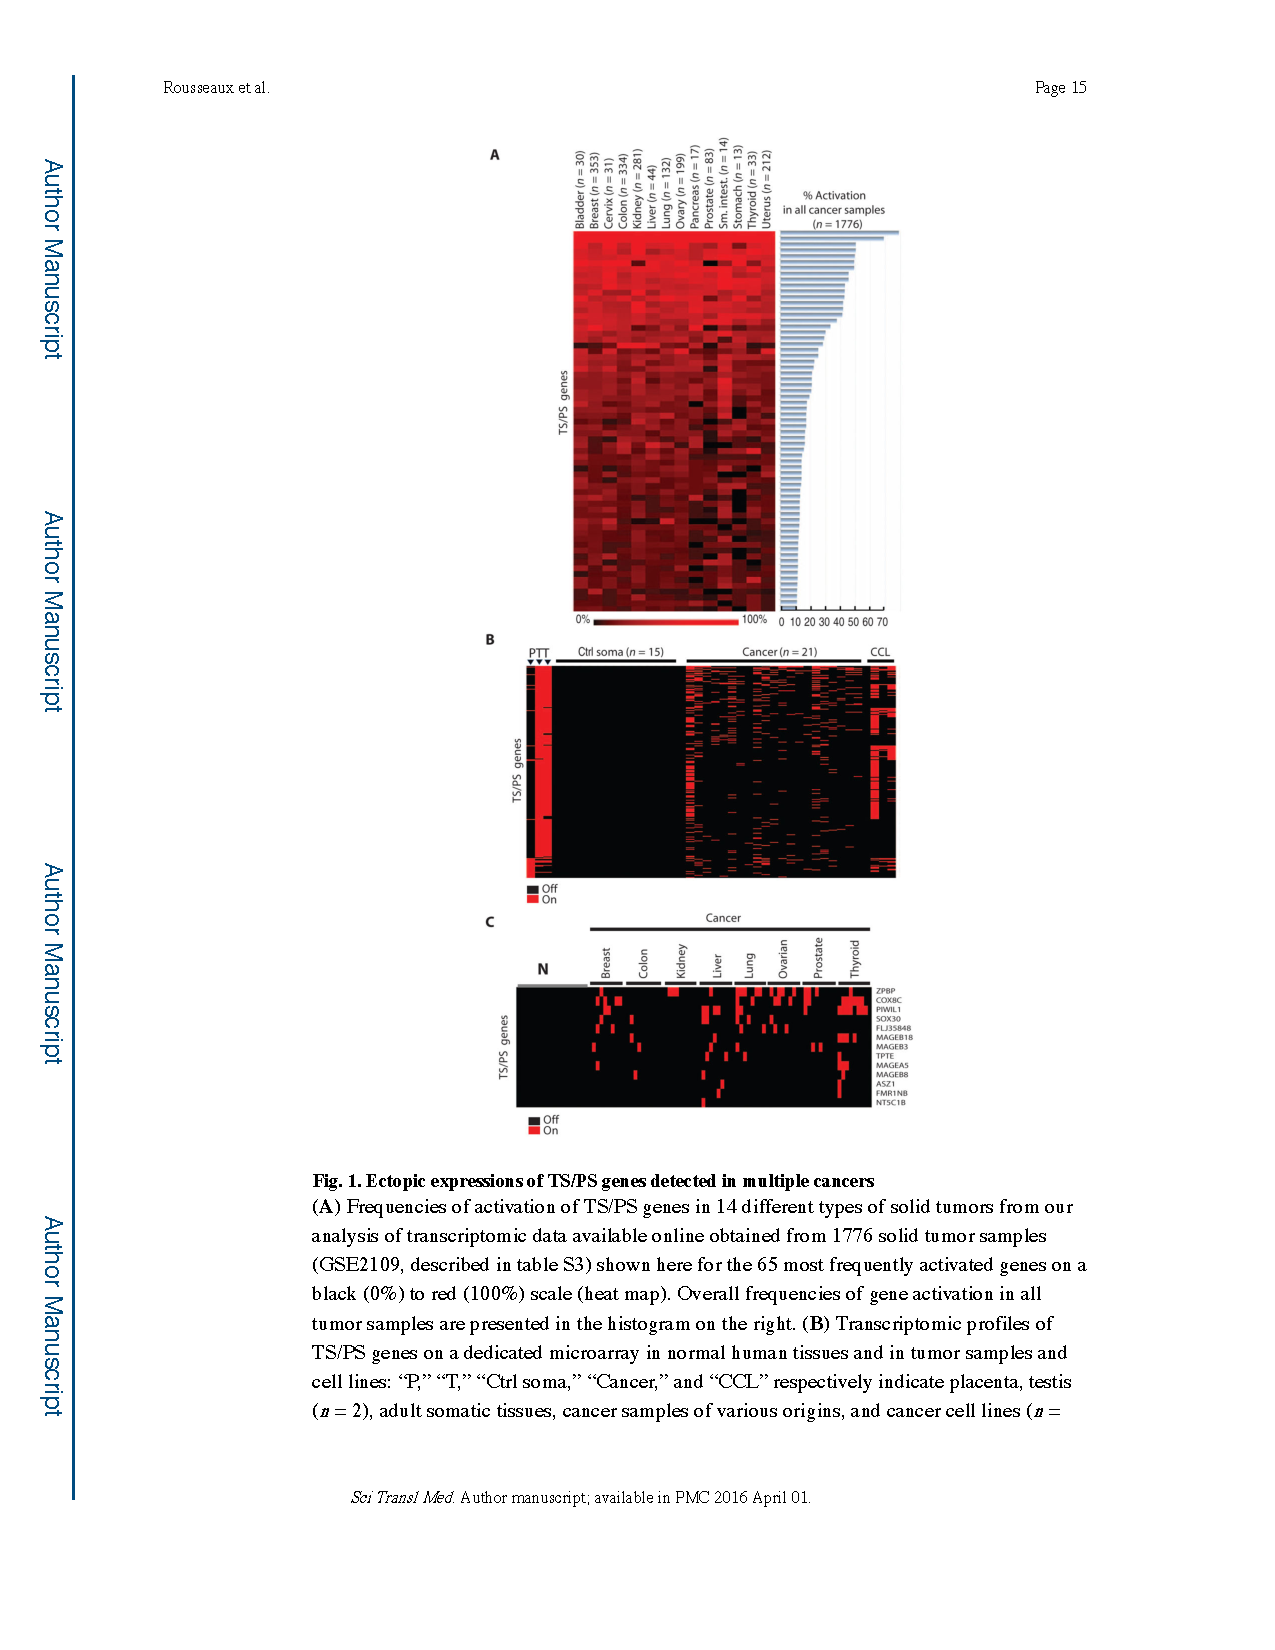
\includegraphics[trim = 85mm 125mm 60mm 107mm, clip, width=.58\linewidth]{figs/fig01}}
\mbox{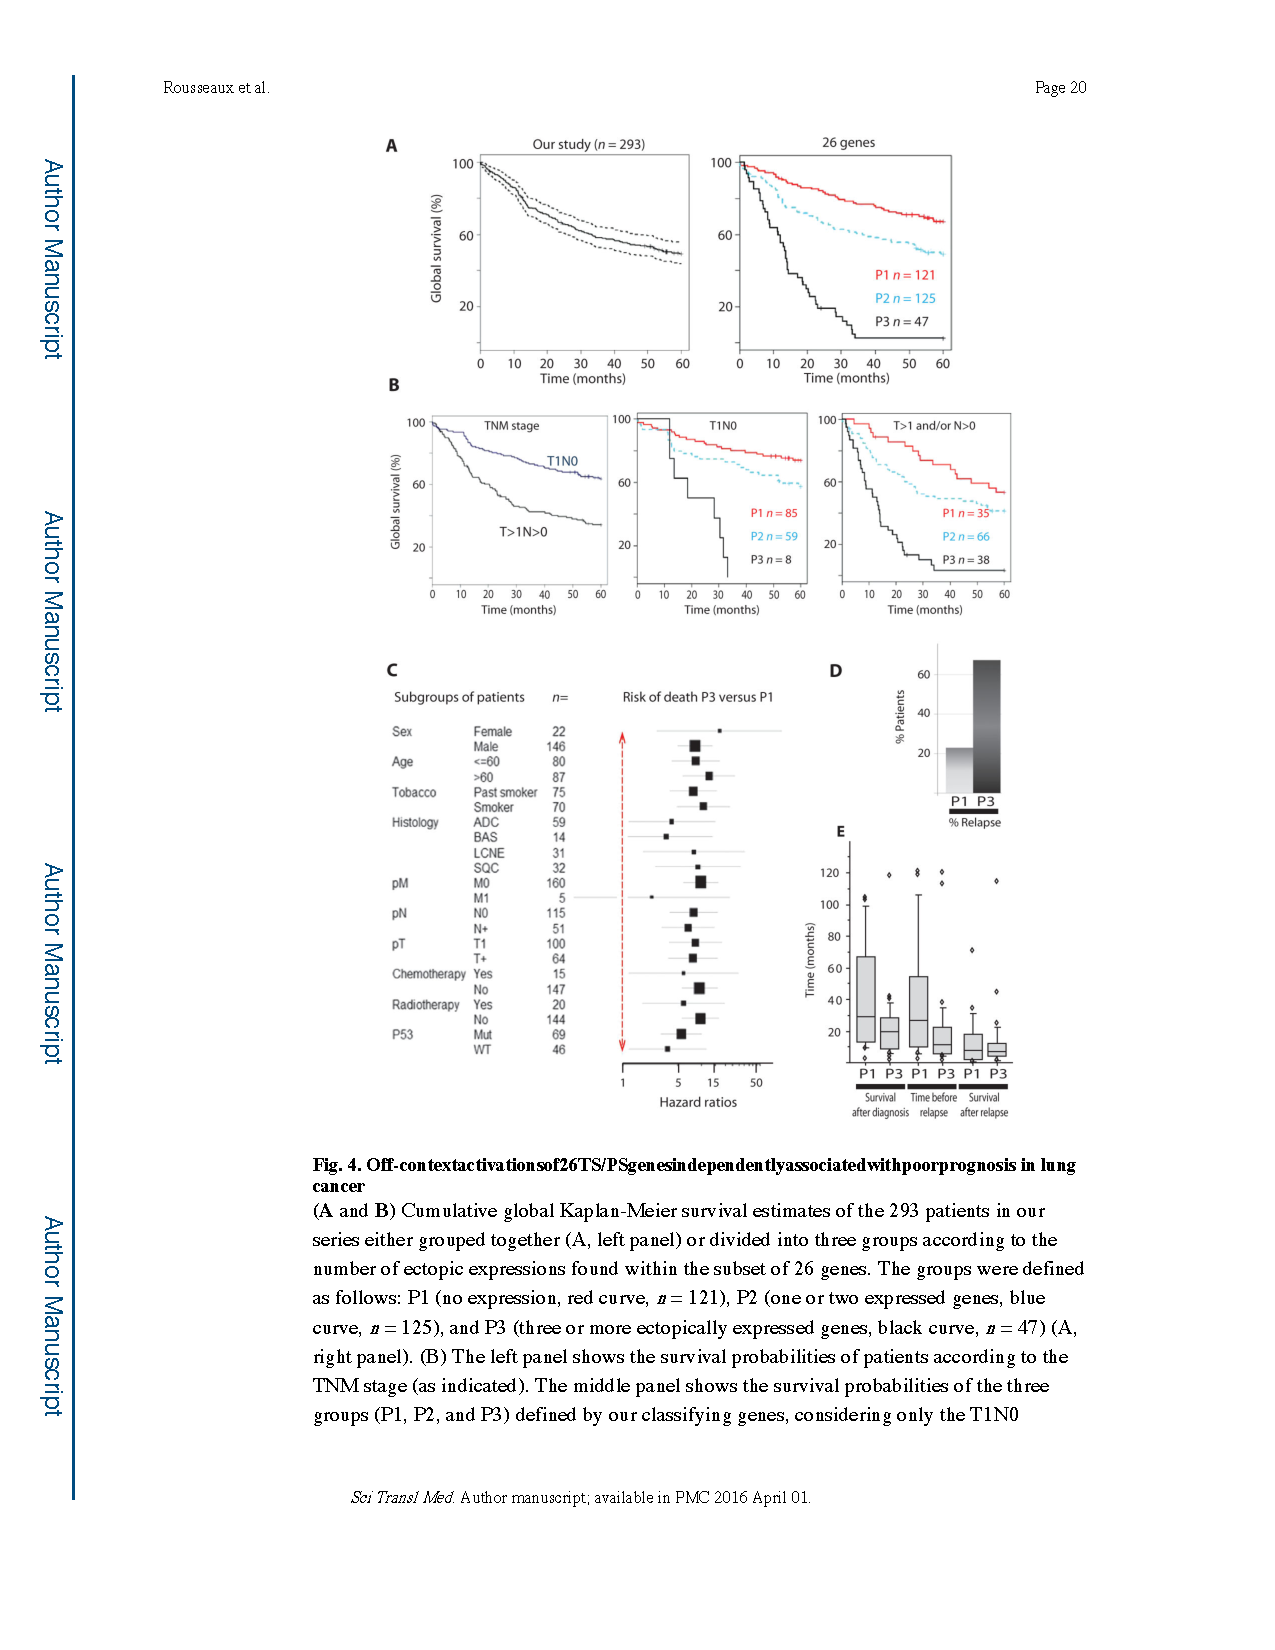
\includegraphics[trim = 120mm 212mm 50mm 20mm, clip, width=.4\linewidth]{figs/fig02}}
}

\begin{center}
\small{\textsl{Left panel: Aberrant activation of testis-specific(TS) and placenta-specific (PS) genes in tumoral lung. Righ panel: Ectopic activation of 26 TS/PS genes is associated with prognosis in lung cancer (Rousseaux et al., Sci Transl Med, 2013).}}
\end{center}

EpiMed \textcolor{RoyalBlue}{\textbf{provides expertise}} in bioinformatics, biostatistics, high performance computing, machine learning and develops \textcolor{RoyalBlue}{\textbf{tools for the community}}:
\begin{itemize}
\item EpiMed Database for clinical data and omics meta-data queries
\item R package “epimedtools” for omics data processing and analysis
\end{itemize}

\end{block}
%----------------------------------------------------------------------------------------


\begin{block}{EpiMed Database}

EpiMed Database provides several tools for clinical, biological and omics data management. The data can be accessed online through web interfaces or programmatically via REST API.

{
\centering
\mbox{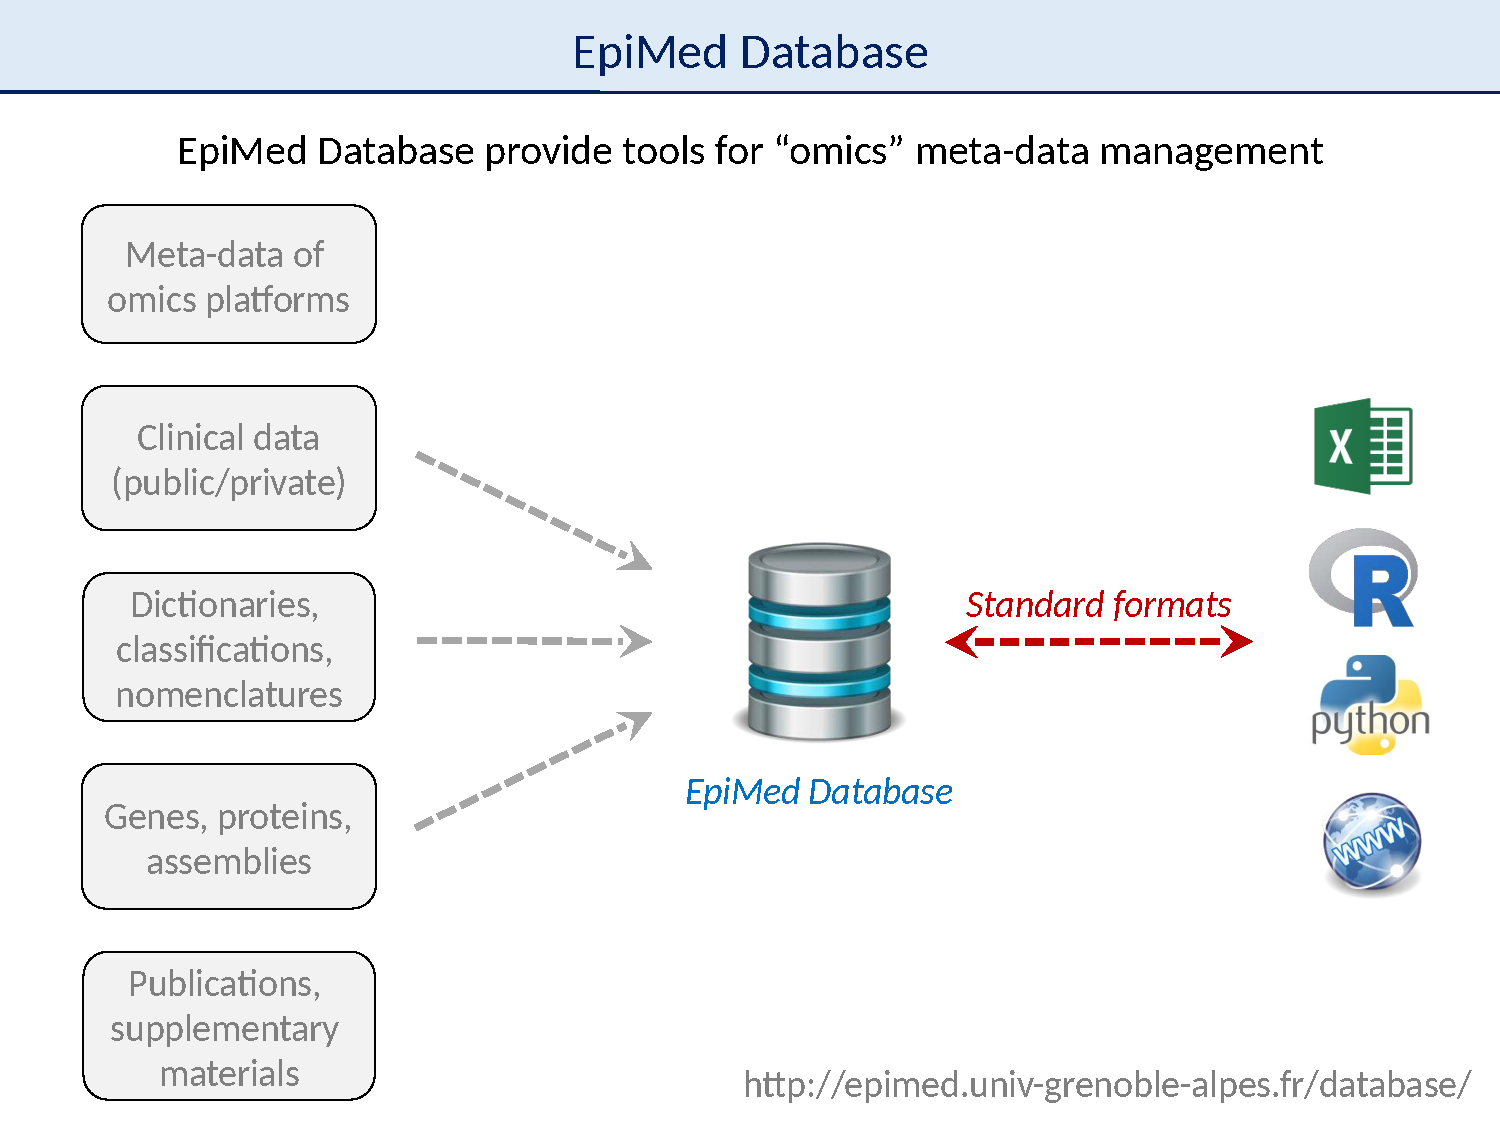
\includegraphics[trim = 0mm 0mm 0mm 30mm, clip, width=\linewidth]{figs/fig03}}

}


\end{block}

\end{column} 

\begin{column}{\sepwid}\end{column} % Empty spacer column

\begin{column}{\twocolwid} % The third column




\begin{block}{Expertise in omics data analysis}

{
\centering
\mbox{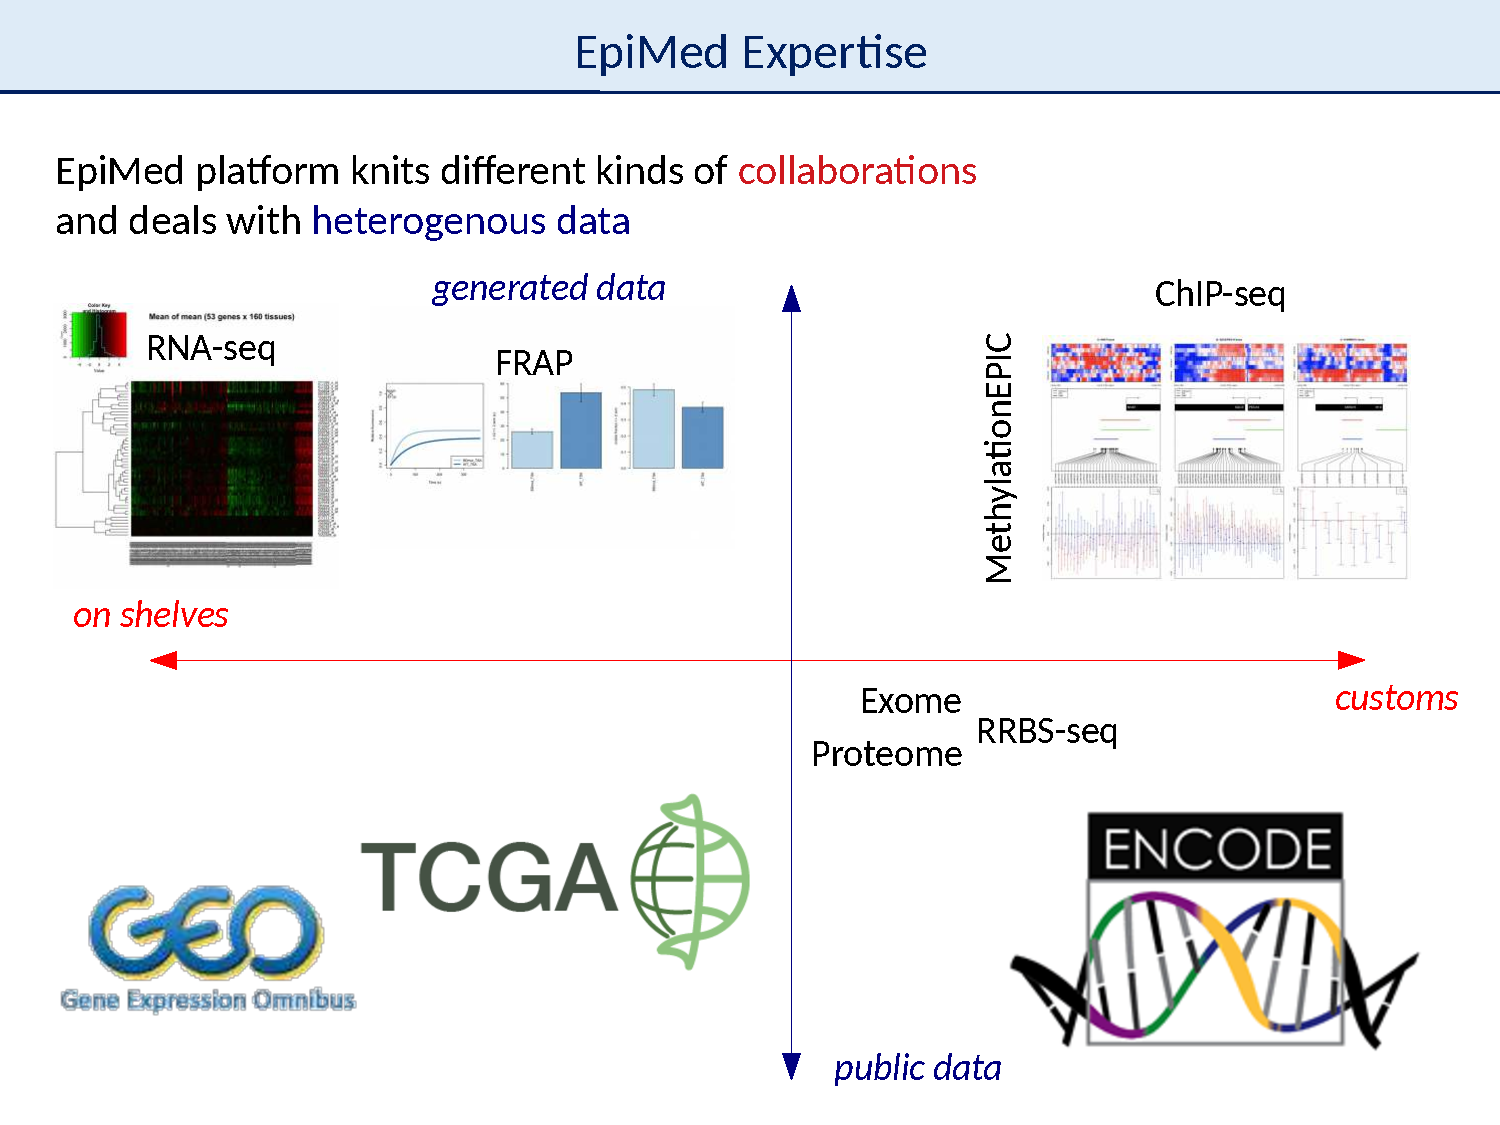
\includegraphics[trim = 0mm 0mm 0mm 43mm, clip, width=.99\linewidth]{figs/fig04}}

}

\end{block}







\begin{block}{Recent projects and collaborations}

\begin{enumerate}
	
	\item \textcolor{RoyalBlue}{\textbf{Identification of highly aggressive tumors by multi-omics analysis in lung adenocarcinoma}}

Beijing -- Shanghai -- Grenoble

\begin{center}
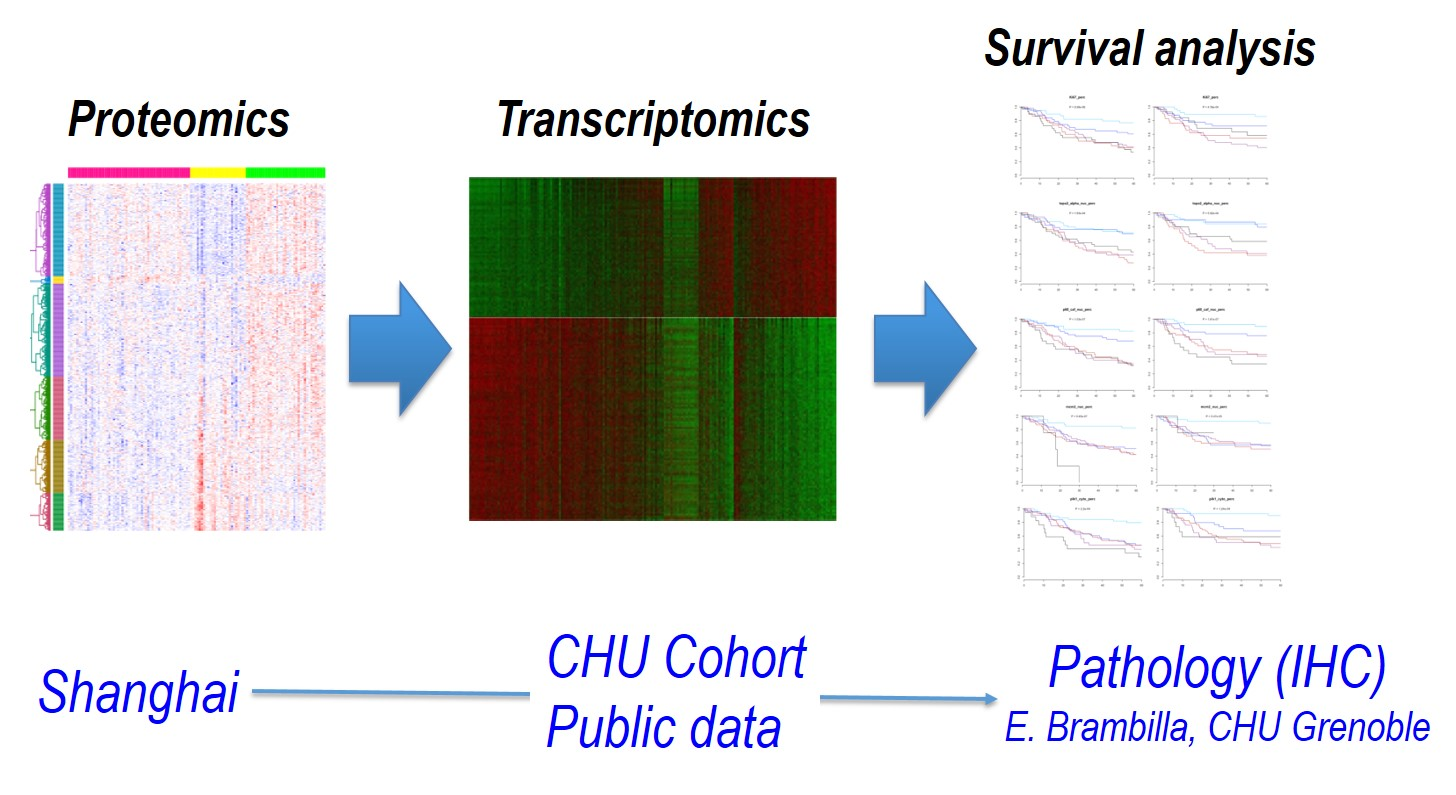
\includegraphics[width=\linewidth]{figs/proteomics_transcriptomics}
\end{center}

\item \textcolor{RoyalBlue}{\textbf{Epigenome-wide association study of placental DNA methylation and maternal smoking status}}

{\justifying
This study shows that tobacco-induced differentially methylated regions (DMRs) in placenta are enriched in epigenetic marks corresponding to enhancer regions, as well as in regions controlling the monoallelic expression of imprinted genes, suggesting mechanisms by which tobacco could impact the epigenome and affect placental development and fetal growth.

}

{
\centering
\mbox{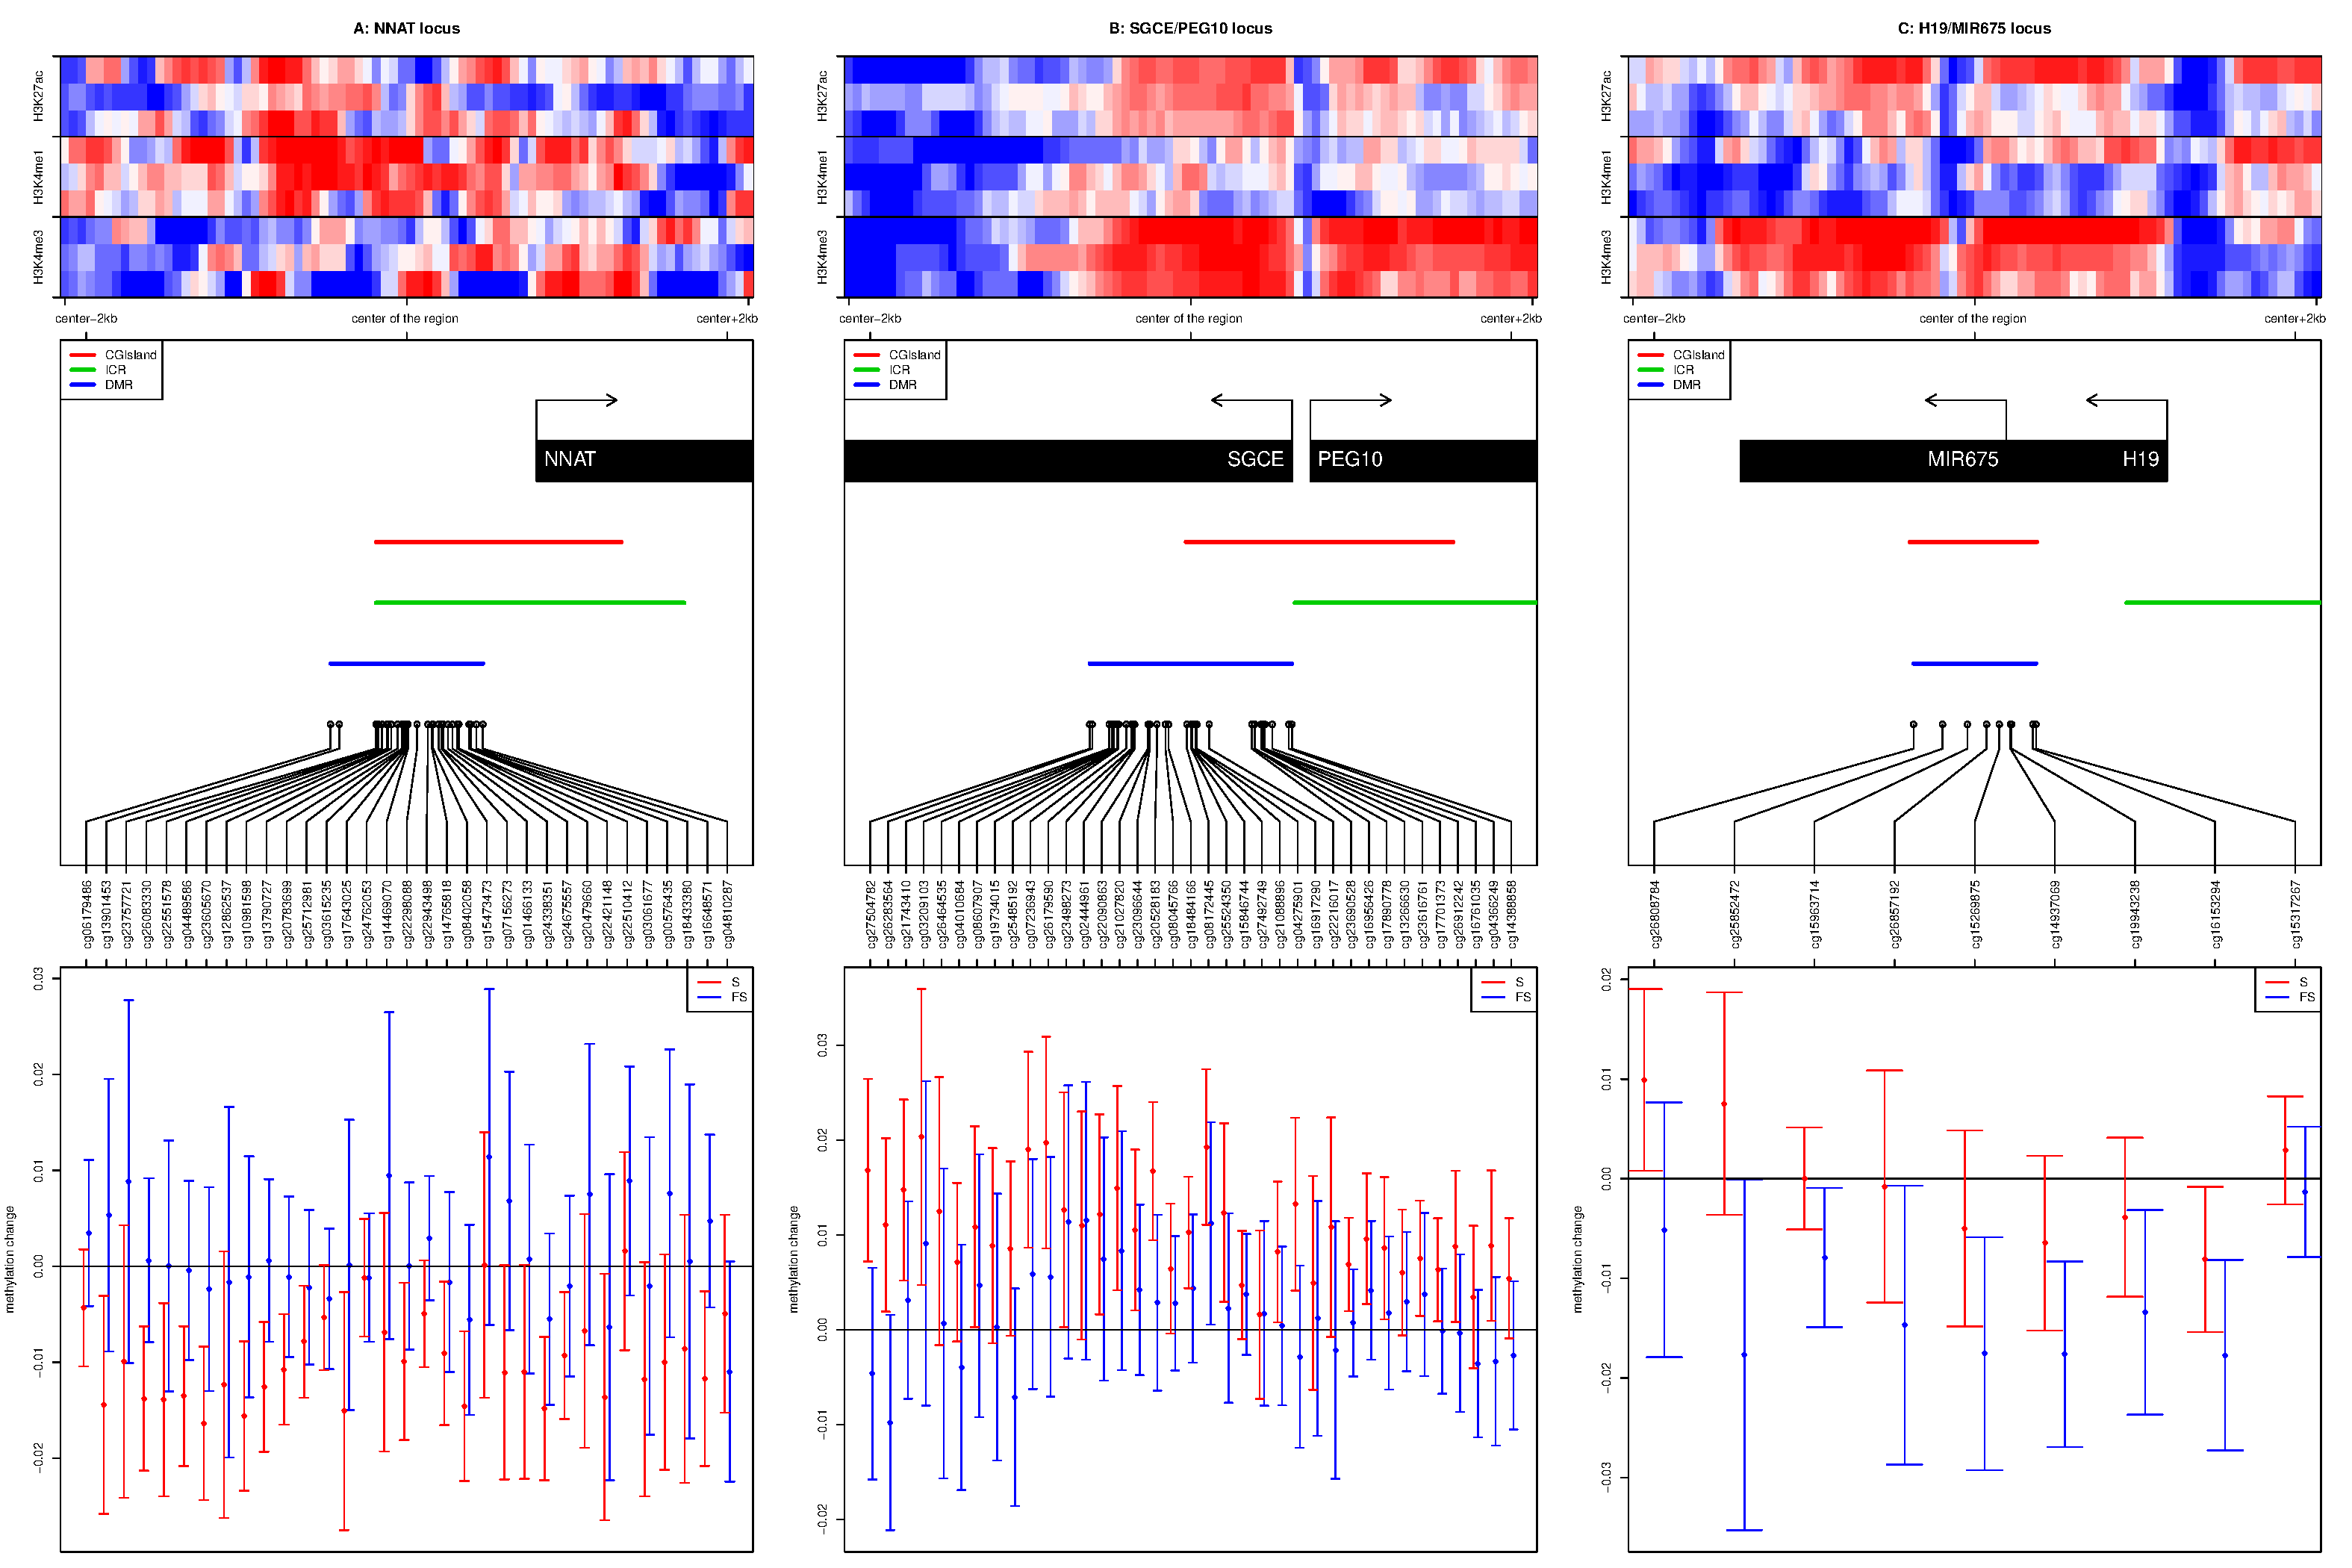
\includegraphics[trim = 0mm 0mm 0mm 0mm, clip, width=.99\linewidth]{figs/fig_3loci}}

}

%The methylation levels of NNAT, SGCE/PEG10 and H19/MIR675 loci are consistently modified following exposure to cigarette smoking.
%The top panels show heatmaps corresponding to H3K4me3, H3K4me1 and H3k27ac enrichments in placenta (ENCODE)
%The middle panels show genes, CGislands, ICR, probes and the DMR we identified.
%The bottom panels show the methylation change in smokers (S) (resp. Former Smokers (FS)) in red (resp. blue) compared to non-smokers. [collab. with J. Lepeule]
\end{enumerate}

\end{block}





% %----------------------------------------------------------------------------------------
% %  REFERENCES
% %----------------------------------------------------------------------------------------
%
% \begin{block}{References}
%
% \nocite{*} % Insert publications even if they are not cited in the poster
% \small{\bibliographystyle{unsrt}
% \bibliography{biblio}\vspace{0.75in}}
%
% \end{block}
%
% %----------------------------------------------------------------------------------------
% %  ACKNOWLEDGEMENTS
% %----------------------------------------------------------------------------------------
%
% \setbeamercolor{block title}{fg=red,bg=white} % Change the block title color
%
% \begin{block}{Acknowledgements}
%
% \small{\rmfamily{
% Funding: The research leading to these results was supported by ITMO Cancer (Plan Cancer 2014-2019, BIO2015-08) and the Grenoble Alpes Data Institute (which is funded by the French National Research Agency under the “Investissements d’Avenir” program ANR-15-IDEX-02).
%
% Most of the computations presented in this paper were performed using the CIMENT/GRICAD infrastructure (https://gricad.univ-grenoble-alpes.fr).
% }} \\
%
% \end{block}
%
% %----------------------------------------------------------------------------------------
% %  CONTACT INFORMATION
% %----------------------------------------------------------------------------------------

 %\setbeamercolor{block alerted title}{fg=black,bg=norange} % Change the alert block title colors
 %\setbeamercolor{block alerted body}{fg=black,bg=white} % Change the alert block body colors
%
%\begin{alertblock}{Contact Information}
%\begin{itemize}
%\item Web: \href{http://epimed.univ-grenoble-alpes.fr/}{http://epimed.univ-grenoble-alpes.fr/}
%\item Email: \href{mailto:iab-epimed@univ-grenoble-alpes.fr}{iab-epimed@univ-grenoble-alpes.fr}
%\item Phone:  +33 (0)4 76 54 95 82
%\end{itemize}
%\begin{center}
%\begin{tabular}{ccc}
%% \includegraphics[width=0.4\linewidth]{logo.png} & \hfill & \includegraphics[width=0.4\linewidth]{logo.png}
%
\includegraphics[trim = 0mm 0mm 160mm 10mm, clip, width=0.25\linewidth]{figs/logo_iab.jpg} & \hfill & 
%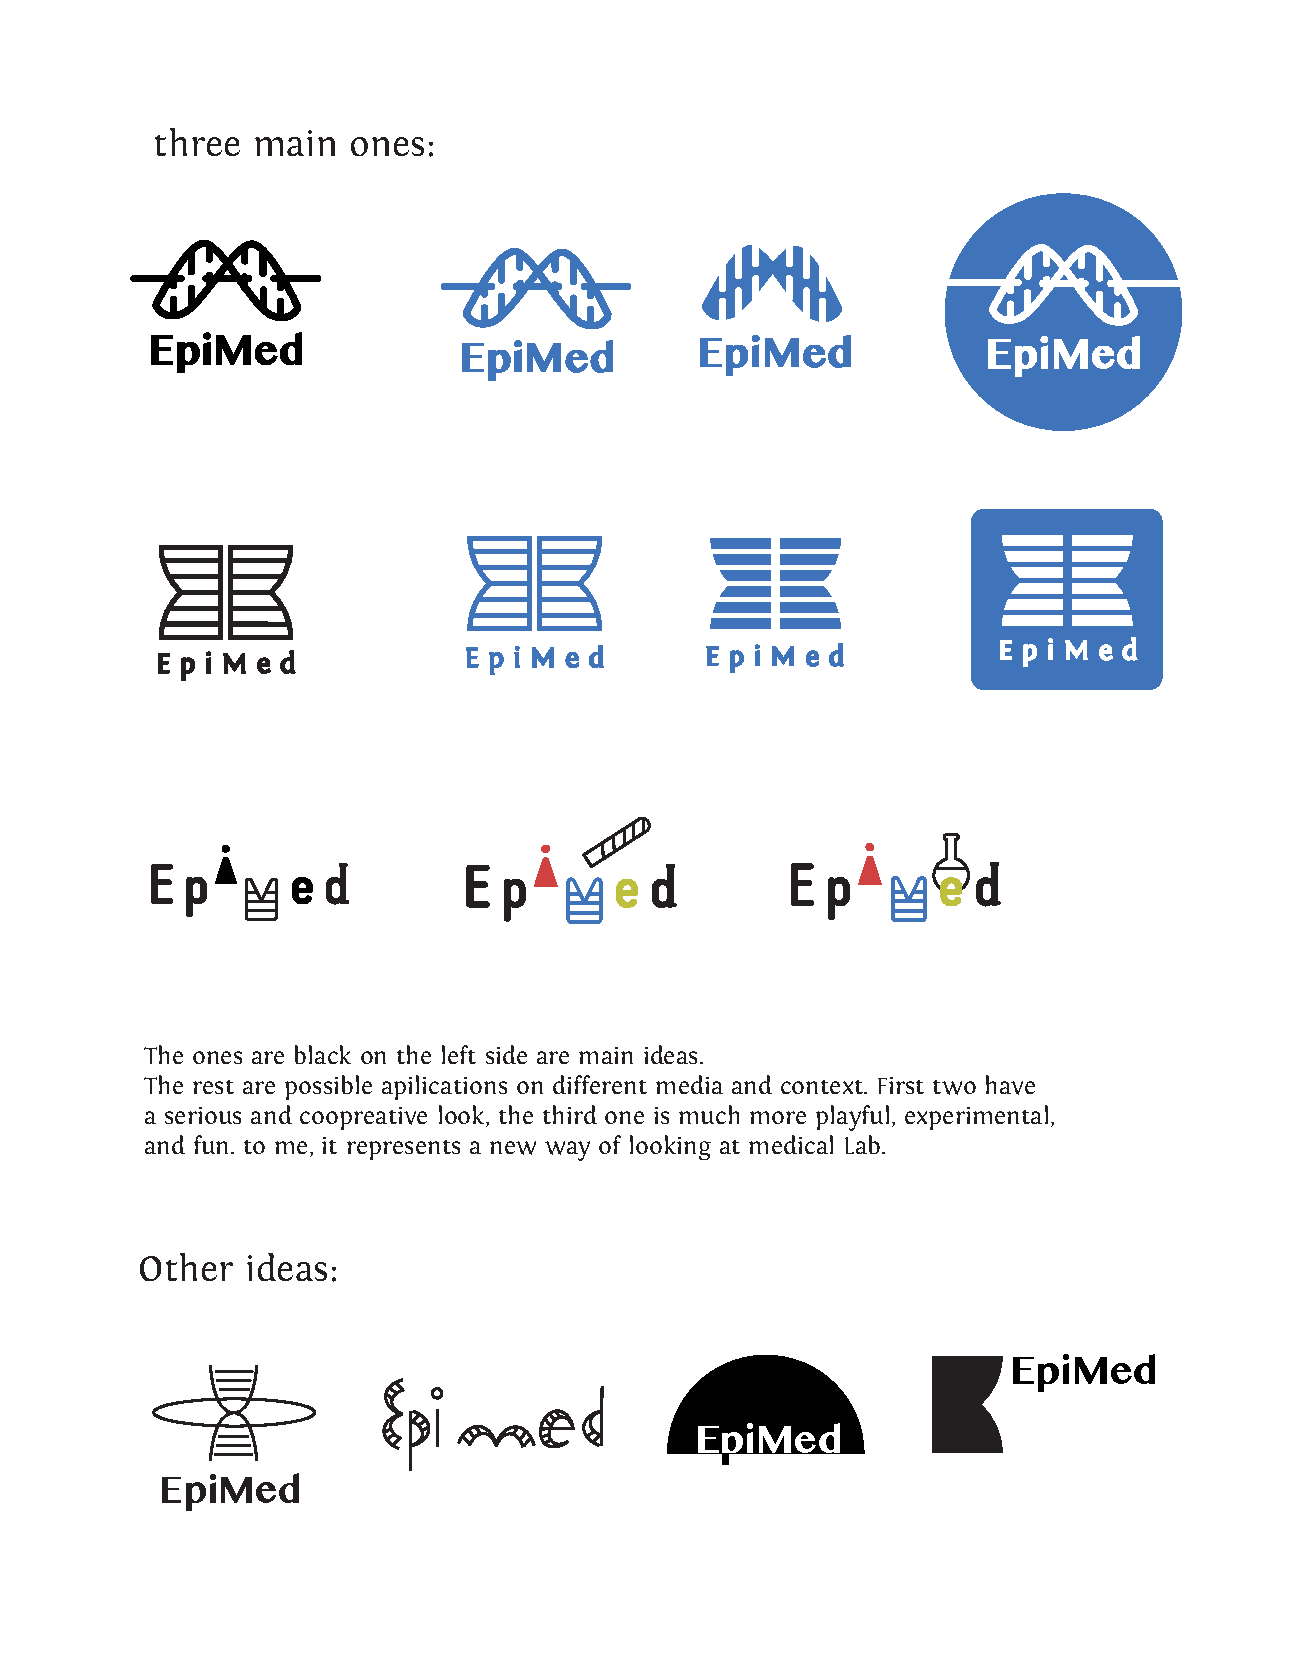
\includegraphics[trim = 150mm 200mm 10mm 32mm, clip, width=0.2\linewidth]{figs/logo_epimed.pdf}
%\end{tabular}
%\end{center}
%
%\end{alertblock}




%----------------------------------------------------------------------------------------

\end{column} % End of the third column

\end{columns} % End of all the columns in the poster

\begin{center}
\textcolor{gray}{E-mail: iab-epimed@univ-grenoble-alpes.fr \hspace{5cm} Web: http://epimed.univ-grenoble-alpes.fr}
\end{center}

\end{frame} % End of the enclosing frame

\end{document}
